\documentclass[dvips,12pt]{article}

% Any percent sign marks a comment to the end of the line

% Every latex document starts with a documentclass declaration like this
% The option dvips allows for graphics, 12pt is the font size, and article
%   is the style

\usepackage[pdftex]{graphicx}
\usepackage{url}
\usepackage{hyperref}

% These are additional packages for "pdflatex", graphics, and to include
% hyperlinks inside a document.

\setlength{\oddsidemargin}{0.25in}
\setlength{\textwidth}{6.5in}
\setlength{\topmargin}{0in}
\setlength{\textheight}{8.5in}

% These force using more of the margins that is the default style

\begin{document}

% Everything after this becomes content
% Replace the text between curly brackets with your own

\title{CS 6630 Project Proposal\\Visualizing SIGGRAPH Publications}
\author{Kui, Wu and Hoang, Duong\\TODO (u0930062)\\TODO@TODO u0933062@utah.edu}
\date{\today}

% You can leave out "date" and it will be added automatically for today
% You can change the "\today" date to any text you like


\maketitle

\section{Introduction and background}
% Basic Info. The project title, your names, e-mail addresses, UIDs, a link to the project repository.
% Background and Motivation. Discuss your motivations and reasons for choosing this project, especially any background or research interests that may have influenced your decision.
When surveying a new field, researchers often want an overview look at the important papers in the field, how they are related, and how popular trends in topics or techniques have been evolving over the years. Traditional search engines such as Google Scholar and digital libraries such as the ACM's can alleviate the task, but only when the researcher has a good idea of what he should look for. Even then, the information obtained from those tools at any given moment is not only too specific but also presented in a non-visual form, making it difficult for the user to see a bigger picture. Being both interested in doing research in computer graphics, in this project we aim to develop a tool to visualize connections between papers published over the years in SIGGRAPH, the most important conference in computer graphics. The tool should show in one place: the citation relationships among SIGGRAPH papers, important papers in each sub-field, prolific authors and their collaboration patterns, popular topics and methods in recent years, and active research institutions in each sub-field. It is our hope that such a tool can be particularly helpful to someone who wants to survey a field and summarize major results. It could also help new researchers in finding not only interesting problems to work on but also pointers to relevant publications for reference. Lastly, prospective graduate students can use information provided by the tool to make more informed decision in their application process.

\section{Project Objectives}
% Project Objectives. Provide the primary questions you are trying to answer with your visualization. What would you like to learn and accomplish? List the benefits.
Our project aims to answer the following questions:
\begin{itemize}
    \item What papers are influential in the field, in terms of citation count?
    \item Given a paper of interest, what papers does it cite? What are the papers citing it?
    \item What topics and techniques are popular, and in which time periods?
    \item Given a set of keywords, what are the most relevant papers/authors/institutions to these keywords?
    \item Who does each author collaborate with the most?
    \item What institutions are more active in a given field, in terms of publication count?    
\end{itemize}
Answering the above questions will put a make a researcher more informed about what papers/authors/topics/techniques to pay more attention to, thereby saving time in the beginning of a survey task. It can also reveal interesting patterns and trends in the past that can help him or her better decide on future research directions for a particular topic of interest.

\section{Data}
% Data. From where and how are you collecting your data? If appropriate, provide a link to your data sources.
Our data comes from multiple sources.
\begin{itemize}
    \item Paper texts are downloaded from the \href{http://dl.acm.org/}{ACM Digital Library}. From these we extract the title, authors and their affiliations, references, and important keywords.
    \item BibTeX information for all papers is downloaded from  the \href{http://dblp.uni-trier.de/db/}{Digital Bibliographic Library Browser}.
    \item Citation count information is queried from \href{https://scholar.google.com/}{Google Scholar}.
\end{itemize}

\section{Data Processing}
% Data Processing. Do you expect to do substantial data cleanup? What quantities do you plan to derive from your data? How will data processing be implemented?
We expect our raw data to require a substantial cleanup process. So far we have collected all the SIGGRAPH papers's pdf files from 2002 to 2015, totaling 17GB of data. These pdf files will be converted to text format, from which we will extract from each paper its title, authors and their affiliations, references and keywords. The extraction process is done using a combination of homemade Python scripts and opensource tools such as \href{http://aye.comp.nus.edu.sg/parsCit/}{ParsCit}.

Meaningful keyword extraction is the most difficult step of the extraction process. Most papers provide a set of "keywords" after the abstract but in our experience, these keywords are not meaningful enough: in any given year, most keywords are used by only one paper. We are looking into using an auto-summarizing tools for this step. Because of the uncertainty of keyword extraction, all features that require keywords will be optional.

We have done cursory testing of our tools and they seemed to be able to extract the required information with high accuracy, thanks to the uniformity in format of the papers. There is still some chance that noise will show up in the extracted data, in which case some post-process cleaning has to be done. We will finally need to remove all non-SIGGRAPH papers from the list of references to make our data more self-contained and easier to work with.

Since our data is highly relational, we plan to store it in an SQL database and query the data with Javascript. At the moment \href{https://github.com/kripken/sql.js/}{sql.js} and \href{https://github.com/mapbox/node-sqlite3}{node-sqlite3} seem to be promising candidates. Tentatively, there will be different tables, one for each of the following: papers, authors, institutions, keywords. Each entry in a table will have necessary fields, for example a paper will contain links to its authors and keywords, an author entry will have links back to his or her papers, and (optionally) links to the institution where he/she worked when a paper was published.

An alternative design is to flatten all the SQL tables into JSON files and load those instead. The SQL approach allows us to not having to load everything into memory at once, perhaps at the cost of more processing time each time users change their query/filter of the data. It is not yet clear to us how big the data will be, and which one of the two approaches will work better.

\section{Visualization Design}
% Visualization Design. How will you display your data? Provide some general ideas that you have for the visualization design. Develop three alternative prototype designs for your visualization. Create one final design that incorporates the best of your three designs. Describe your designs and justify your choices of visual encodings. We recommend you use the Five Design Sheet Methodology.
Our design will consist of four different views (Fig. \ref*{fig:overview}):

\begin{figure}[htb!]
    \centering
    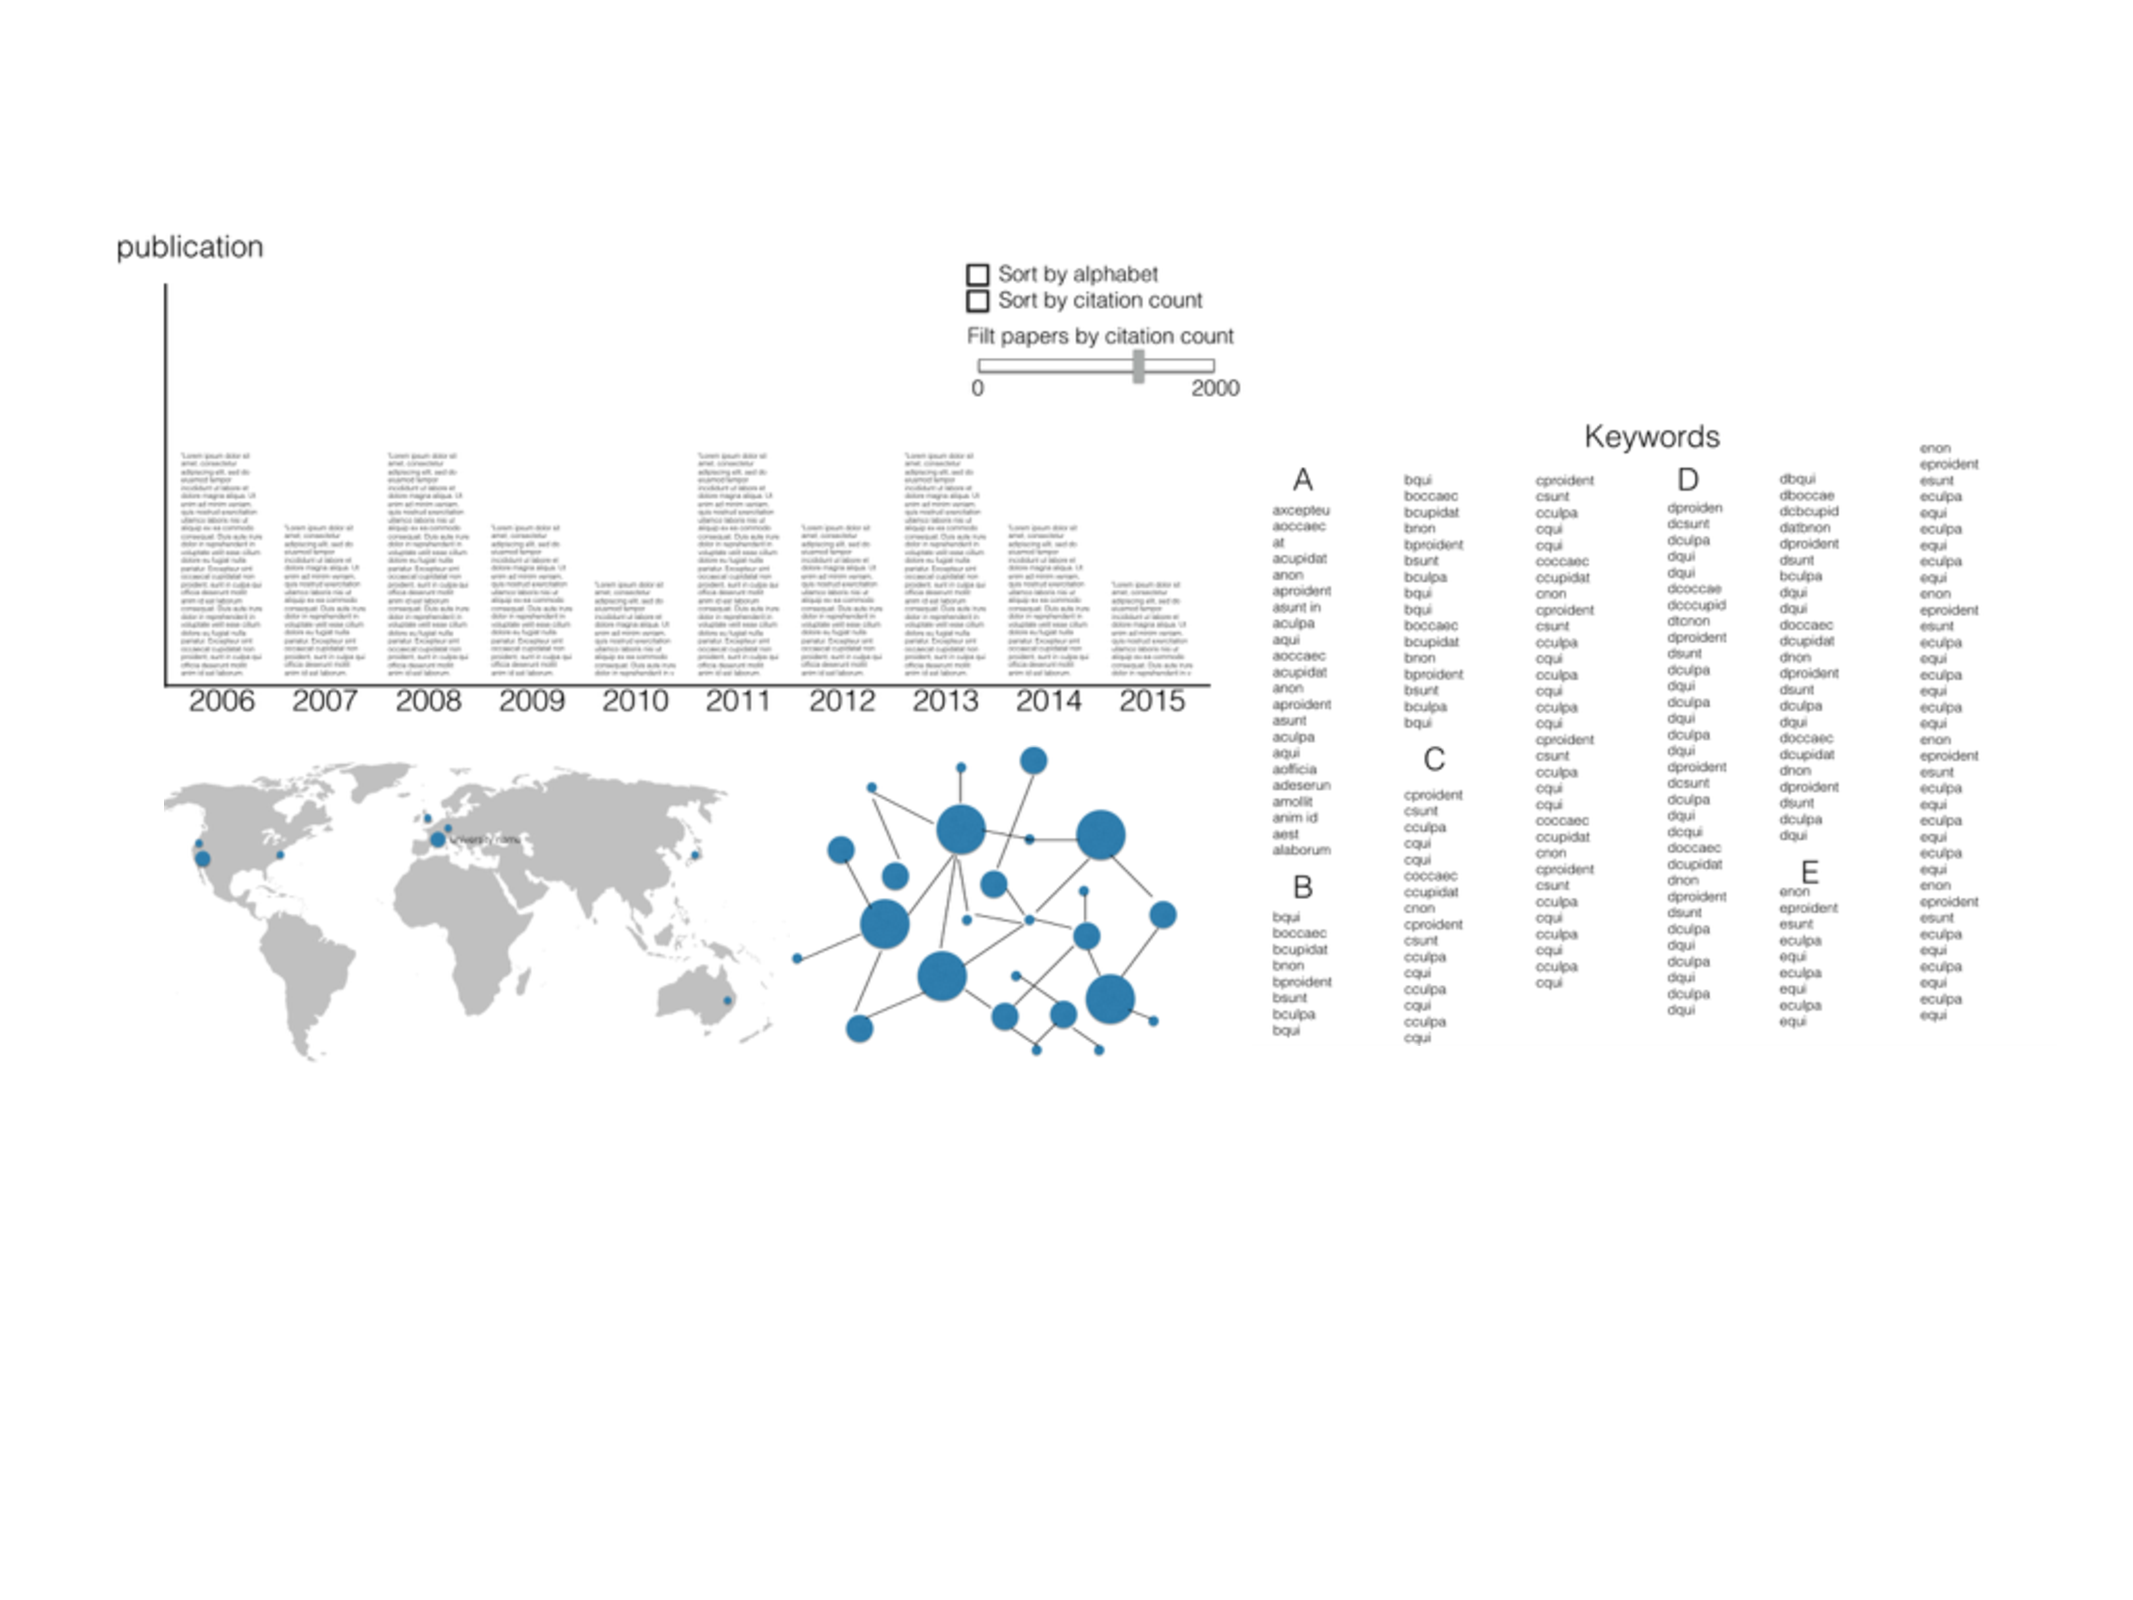
\includegraphics[width=\paperwidth]{visproposalDrawing_page_Part_1.pdf}
    \caption{Overview}
    \label{fig:overview}
\end{figure}

\textbf{Paper view (the main view)}. Here we show all the papers, grouped by year. Each year occupies one column. This view will be wide enough to show about ten years but will be scrollable horizontally to move the focus to a different period of time. Each paper's title will appear on one row and be click-able. When a paper is clicked on, the papers that this paper cites and the ones that cite it will be highlighted (Fig. \ref{fig:paper_view}). Moreover, when a paper is moused over, a pop-up will show the paper's full title, author lists, keywords, and DOI link (Fig. \ref{fig:pop-up}). A bar will appear right under each paper's title, the length of which is proportional to the paper's number of citations (this is not yet shown in our design sketches). This help the user identify influential papers at a glance. The whole view can be sorted either alphabetically or by citation count. The papers can also be filtered by citation count, to hide papers with lesser impacts.

\begin{figure}[htb!]
    \centering
    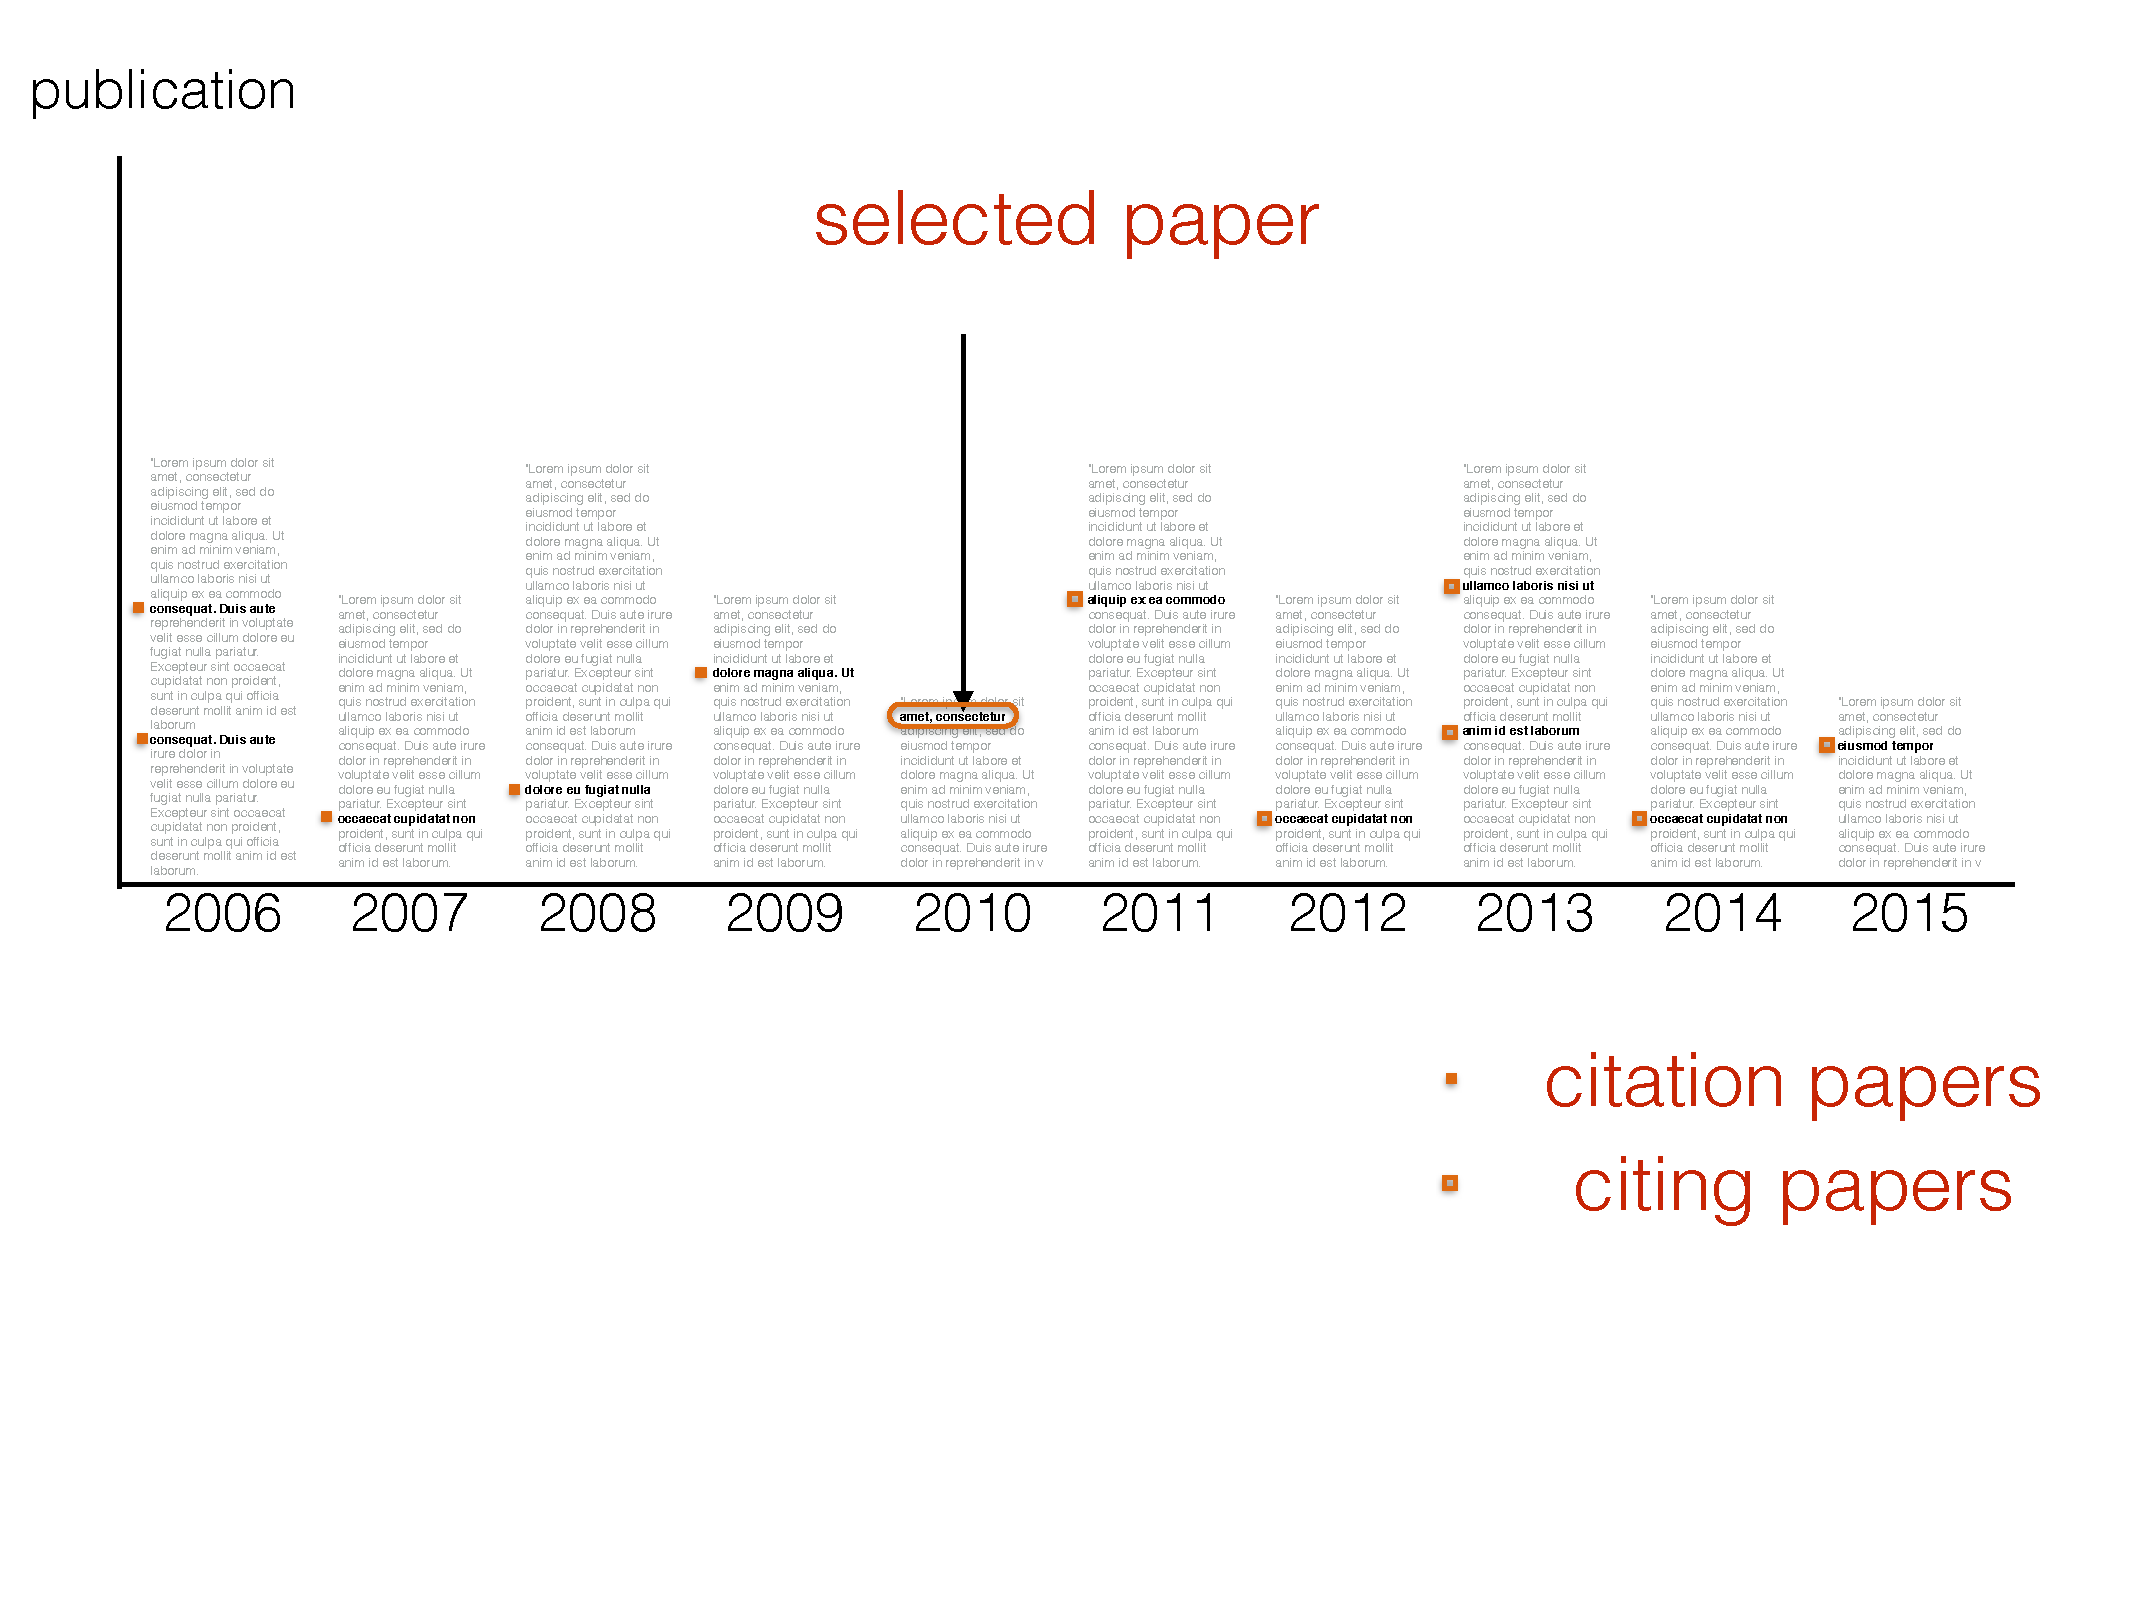
\includegraphics[width=\paperwidth]{visproposalDrawing_page_Part_2.pdf}
    \caption{Paper view}
    \label{fig:paper_view}
\end{figure}

\begin{figure}[htb!]
    \centering
    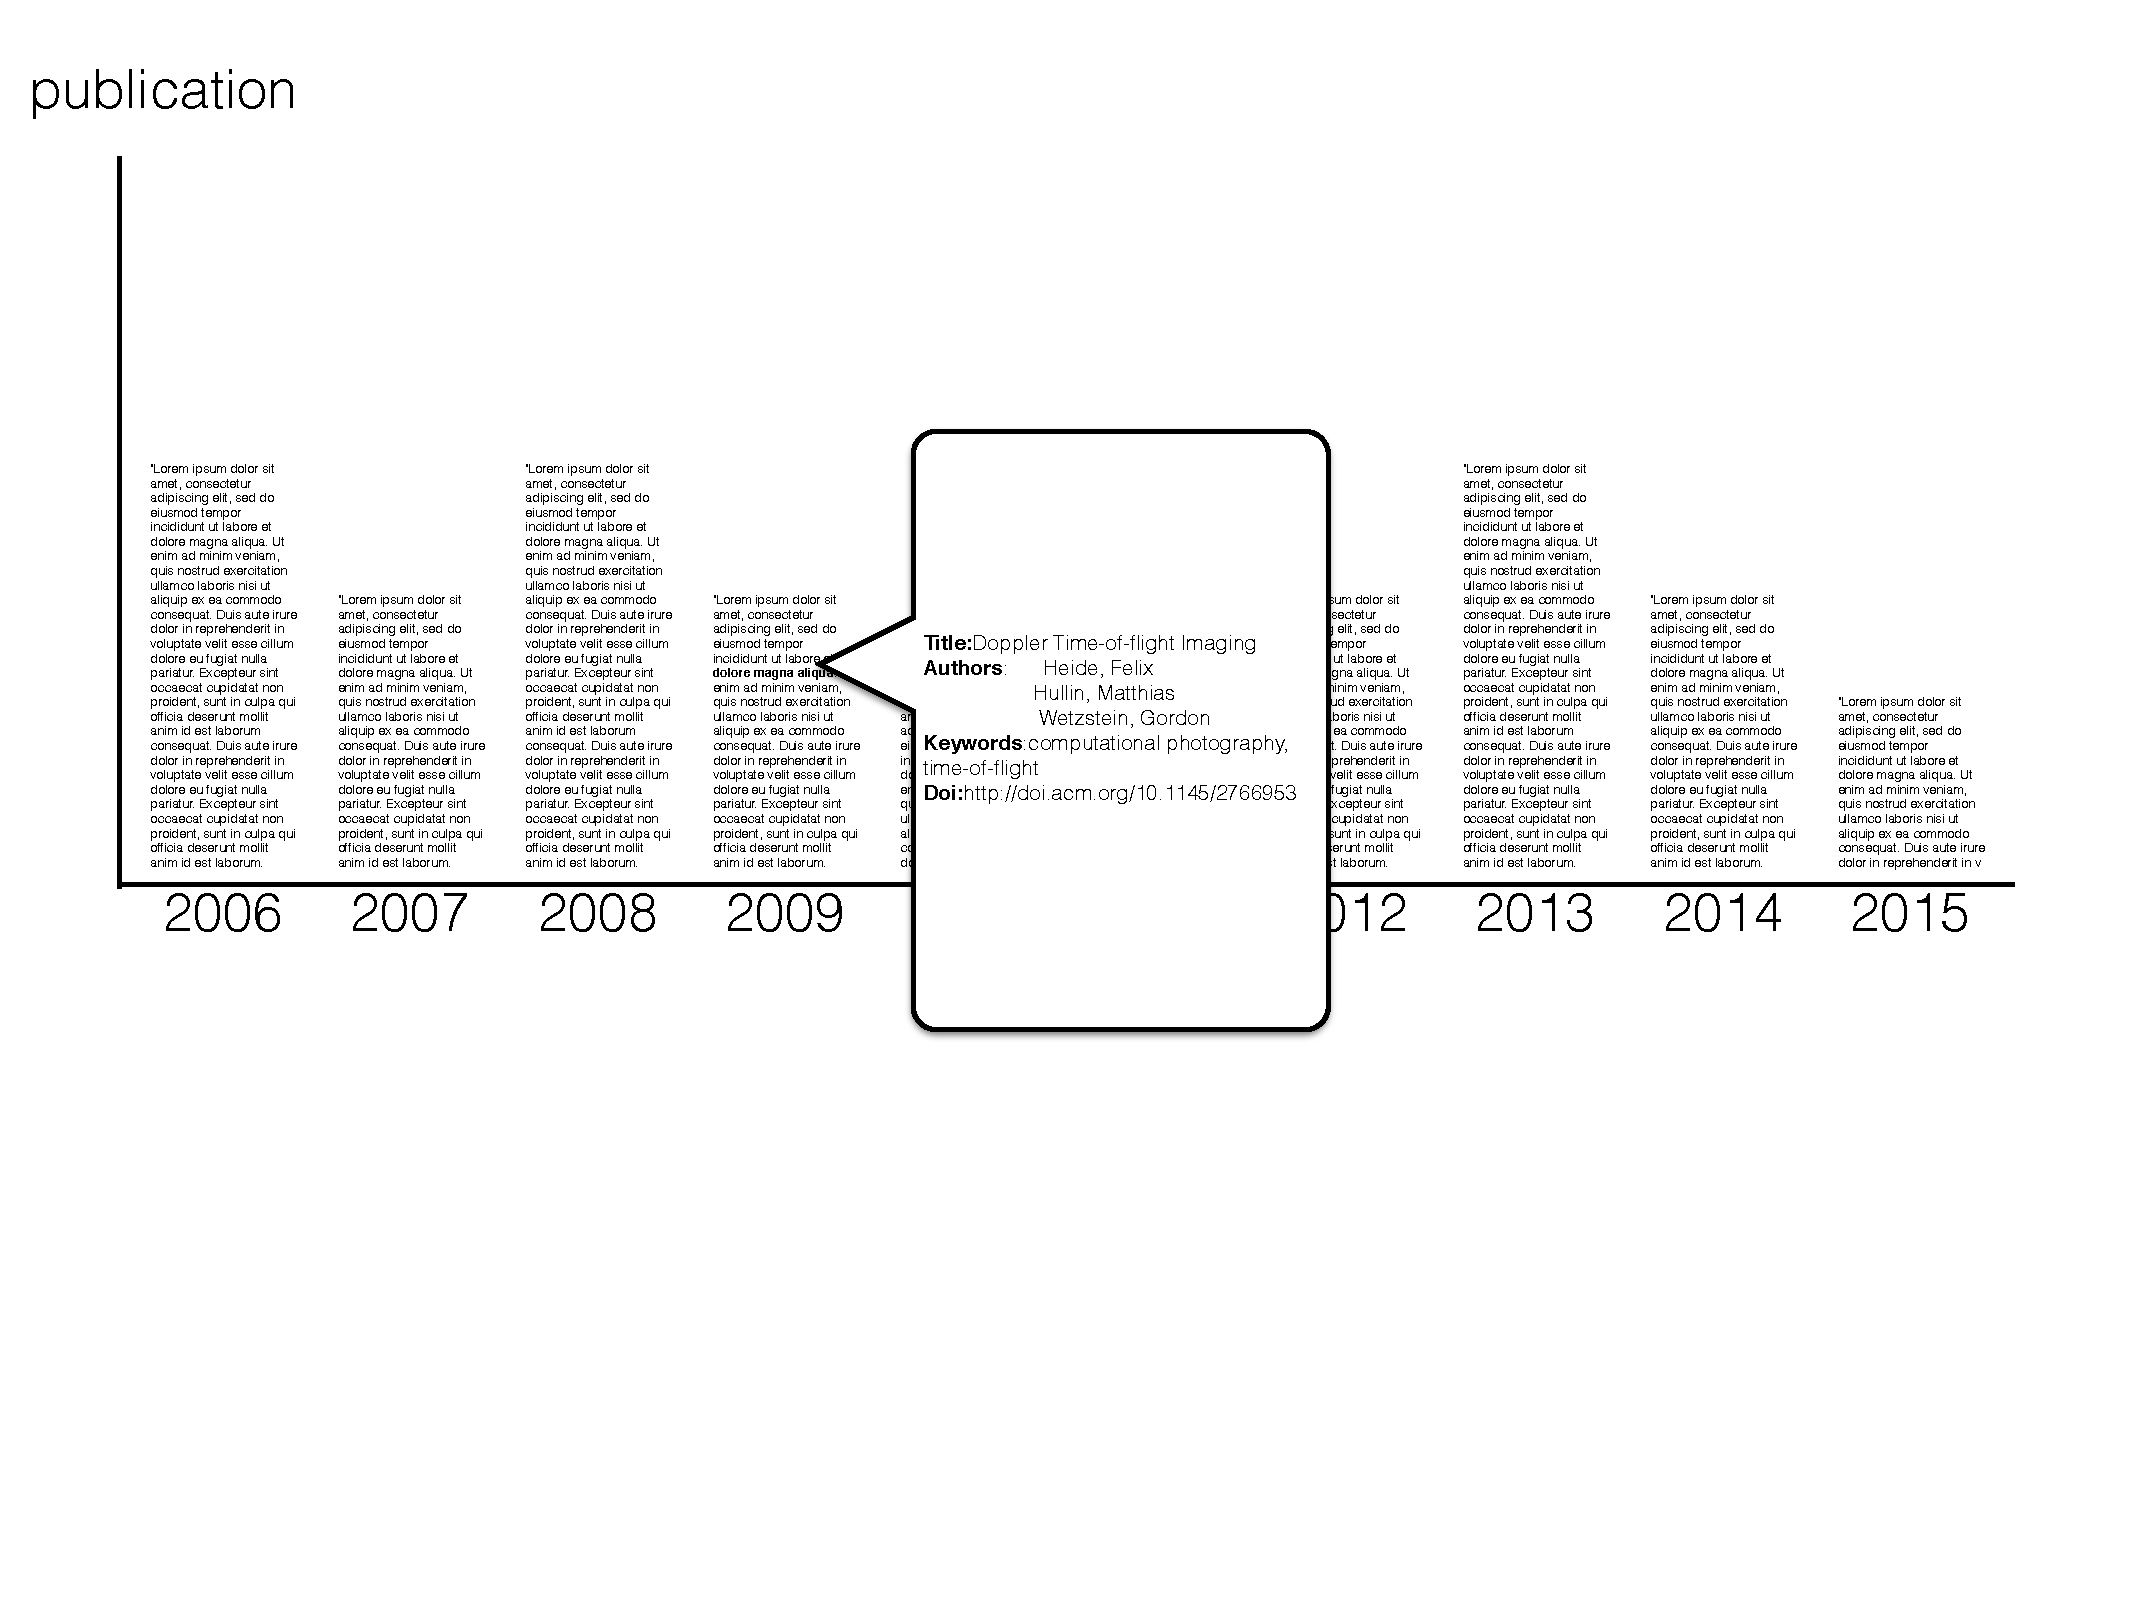
\includegraphics[width=\paperwidth]{visproposalDrawing_page_Part_8.pdf}
    \caption{Paper details pop-up}
    \label{fig:pop-up}
\end{figure}

\textbf{Institution view}. Here we show a map of all the institutions that have published papers to SIGGRAPH. They will appear as circles on a projected world map. The bigger the circle is, the more publications that institution has in the selected time period. Mousing over an institution will show its name and address.

\textbf{Author view}. In this view we show all paper authors and their collaboration relationships as a node-link diagram. Each author is a node, and two authors are linked if they have written a paper together. Bigger nodes represent more prolific authors, in terms of some metrics such as the H-index. Mousing over an author will show his/her name and affiliations.

\textbf{Keyword view}. 

\textbf{Interaction between views}.

\section{Features}
\subsection{Must-Have Features}
% Must-Have Features. List the features without which you would consider your project to be a failure.
\subsection{Optional Features}
% Optional Features. List the features which you consider to be nice to have, but not critical.

\section{Project Schedule}
\begin{itemize}
	\item Week 10: Process data
	\begin{itemize}
		\item Extract data, such as citation counts and affiliations, from papers and Google Scholar.
		\item Create an SQL database based on the extracted data.
	\end{itemize}
	\item Week 11: Create a basic framework
	\begin{itemize}
		\item Create ``Author'' view, ``Paper'' view, and ``Institution'' view.
	\end{itemize}
	\item Week 12: Project Milestone due
	\begin{itemize}
		\item Create interactions between views. Selecting a element in one view will update the other views accordingly.
	\end{itemize}
	\item Week 13: Optimization
	\begin{itemize}
		\item Optimize interaction speed if necessary
		\item Improve the aesthetic and visual coherency of the design
	\end{itemize}
	\item Week 14: Extract keywords 
	\begin{itemize}
		\item Extract keywords and insert them into the database
		\item Create ``Keyword'' view and link it to the others views
	\end{itemize}
	\item Week 15: Final Project due
	\begin{itemize} 
		\item Improve the project based on the instructor's feedbacks 		
	\end{itemize} 
\end{itemize}
% Project Schedule. Make sure that you plan your work so that you can avoid a big rush right before the final project deadline, and delegate different modules and responsibilities among your team members. Write this in terms of weekly deadlines.

\end{document}